\scanpage{133}

c) Soit $X$ un schéma \deleted{complet}\inserted{propre} sur un corps $k$, supposons $H^{\unsure{0|o}}(X,\underline{O}_{X})=k$. La catégorie $\inserted{C}$ des faisceaux cohérents sur $X$ est une catégorie avec $\otimes,\handwritten{\phi},\handwritten{\psi},$ \deleted{Hom} $1$, \uline{Hom} internes, \inserted{\handwritten{$\mathrm{Hom}(X,Y)$ de dim. finie sur $k$,}}\figure{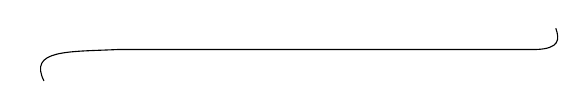
\begin{tikzpicture}[baseline=-.6ex,x=1cm,y=1cm]
\draw (.05,-.25) .. controls (-.15,.15) and (.35,.12) .. (1,.15) -- (6.3,.15) .. controls (6.6,.16) and (6.6,.28) .. (6.55,.42);
\end{tikzpicture}} mais l'homomorphisme $\overset{\handwritten{\vee}}{X}\otimes Y\handwritten{\simeq}\underline{\mathrm{Hom}}(X,Y)$ \uline{n'est pas un isomorphisme}\inserted{(axiome de rigidité)}\figure{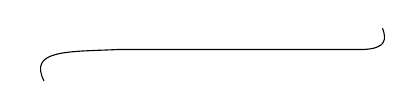
\begin{tikzpicture}[baseline=-.6ex,x=1cm,y=1cm]
\draw (.05,-.25) .. controls (-.15,.15) and (.35,.12) .. (1,.15) -- (4.1,.15) .. controls (4.4,.16) and (4.4,.28) .. (4.35,.42);
\end{tikzpicture}}. C'est pour cela qu'il n'y a pas lieu de s'attendre à une vraie théorie de Galois de $\deleted{X}C$. Il y a des foncteurs fibres associés aux divers points de $X$ (pas nécessairement fermés), à $x$ correspond un foncteur fibre défini sur $k(x)$; sans doute\deleted{i} il n'y en a pas d'autres à isomorphisme près (à vérifier). Ils\deleted{\unsure{o|e}} ont toutes les compatibilités, mais \uline{ils ne sont pas exacts}, \deleted{Pour y rém} \uline{ni fidèles}. Pour rémédier au défaut d'exactitude, sans que $C$ cesse d'être abélienne (sinon on prendrait les Modules loc. libres seulement !), on peut se fixer un ouvert $U\quad X$ et définir $C$ en prenant des \unsure{\deleted{f}F|F}aisceaux cohérents qui, sur $U$, sont munis d'une stratification relative\deleted{e}ment à $k$: tout point $x\handwritten{\in}\deleted{M}U$ fournit un foncteur fibre exact. Cependant, si $U\handwritten{\not}=X$, ce foncteur ne sera pas fidèle. Bien sûr, si $U=X$, l'áxiome de rigidité est satisfait, et on sait qu'on a une théorie de Galois. Il doit résulter de cette dernière que $C$ n'a pas de foncteur fibre (compatible avec toutes les données) sur une extension de $k$ (car autrement l'axiome de rigidité serait \rlap{s}\kern.35em atisfait).

\uline{A prouver:} Soit $C$ une catégorie \inserted{abélienne}\figure{\begin{tikzpicture}[baseline=-.6ex,x=1cm,y=1cm]
\draw (.05,-.25) .. controls (-.15,.15) and (.35,.12) .. (1,.15) -- (1.7,.15) .. controls (2.0,.16) and (2.0,.28) .. (1.95,.42);
\end{tikzpicture}} avec $\otimes_{\deleted{\unsure{k|1|x}}}$ biadditif, $\handwritten{\phi},\handwritten{\psi},1,{}^{\handwritten{\vee}}$ et rigidité. Alors a) $\inserted{k=}\mathrm{End}(\unsure{\deleted{4}1|\deleted{k}1|\mathbb{1}|1})$ est un anneau absolument plat, donc un composé fini de \deleted{\unsure{orops|orcps}} corps s'il est noethérien. b) Les $\mathrm{Hom}(\deleted{C}X,Y)$ sont des modules de présentation finie \inserted{i.e. cohérents}\figure{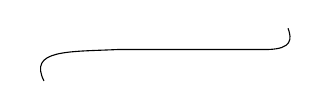
\begin{tikzpicture}[baseline=-.6ex,x=1cm,y=1cm]
\draw (.05,-.25) .. controls (-.15,.15) and (.35,.12) .. (1,.15) -- (2.9,.15) .. controls (3.2,.16) and (3.2,.28) .. (3.15,.42);
\end{tikzpicture}} \deleted{(}sur $k$ (NB les modules de présentation finie sur $k$ forment une catégorie abélienne, en fait $k$ est un anneau ``cohérent''\unsure{\deleted{,})|)}. c) \deleted{Toute sous-catégorie de $C$ stable par tout et à \unsure{engend}} $C$ est limite inductive de sous-catégories (en gén\handwritten{\unsure{é|\deleted{u}é}}ral pas pleines) stables par tout, y compris noyaux, conoyaux, ${}^{\handwritten{\vee}}$, $\otimes$, et correspondants à des anneaux $k_{i}$ qui sont des \deleted{sommes} composés de corps. d) Le cas d'un composé de corps se ramène à celui d'un corps.
